% !TeX spellcheck = en_US
\chapter{Implementation}\label{ch:implementation}


\section{Two-dimensional Decision Function} \label{sec:2D}

Function \ref{eq:2D_g} determines the limit state. Both random variables follow a normal distribution with mean \(0\) and standard deviation \(1\).

\begin{equation} \label{eq:2D_g}
	g(x_1, x_2) = 2 - x_2 + \exp{\bigg ( - \frac{x_1^2}{10} \bigg )} + \bigg ( \frac{x_1}{5} \bigg )^4
\end{equation}

The figure \ref{fig:2D_SVM} shows all the samples (\(10^6\)). Each ordered pair was evaluated in the limit state function \ref{eq:2D_g}. If less than zero it was classified as unsafe, otherwise it was classified as safe.

This simulation gives a probability of failure \(P_f = 1.7 \times 10^{-3}\). At first glance it would appear that the proportion of points that fail would be much higher. However, it should be noted that a large number of points are overlapping in a very dense area. Therefore, conclusions should not be hastily drawn just by looking at the graph.


\begin{figure}
	\myfloatalign
	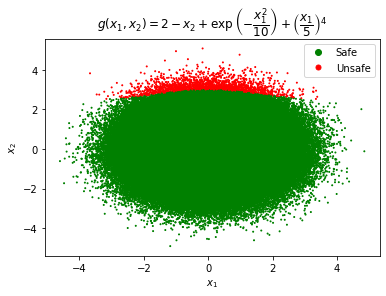
\includegraphics[width=0.7\linewidth]{gfx/2D_MCS}
	\caption{Normal random samples and their classification}
	\label{fig:2dmcs}
\end{figure}

On the other hand, \(10^4\) uniformly distributed samples evaluated on the limit state function were used to train the \ac{SVM} algorithm although the majority of them were not taken into account as they were not close enough to the margin to be useful.

To initialize the algorithm, one point from each of the two categories was required. The points \((x_1, x_2)\) chosen were \((0,0)\) which is safe and \((0,4)\) which is unsafe.

A \ac{RBF} kernel (see equation \ref{eq:RBF_gamma}) with \(\sigma = \sqrt{5}\) was used. For the calculation of the gamma parameter, the equation \ref{eq:RBF_gamma} was slightly modified for a better fit \( \left ( \gamma = \tfrac{1}{1.5 \sigma^2} \right) \) as it is a free parameter.

\begin{figure}
	\myfloatalign
	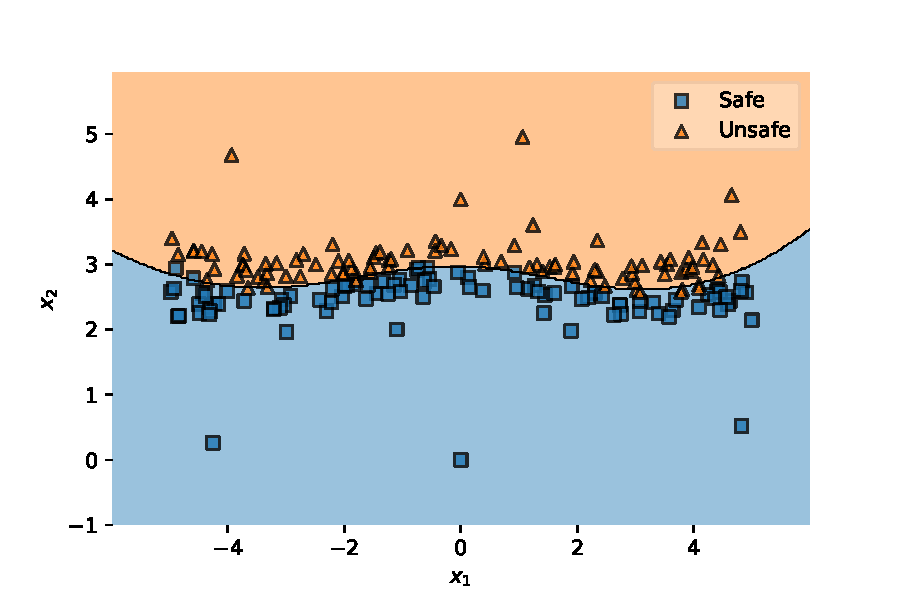
\includegraphics[width=0.7\linewidth]{gfx/SVM_1e4_1e6}
	\caption[SVM implementation]{SVM implementation with actual categories and decision function}
	\label{fig:2D_SVM}
\end{figure}

Figure \ref{fig:2D_SVM} shows the points that trained the model. They are identified with their actual category and additionally the decision function (a hyperplane in a higher dimension) can be seen. The model ended up with 463 support vectors: 235 safe and 228 unsafe.

\begin{figure}
	\myfloatalign
	\includegraphics[width=0.7\linewidth]{gfx/SVM_1e4_1e6_matrix}
	\caption{Confusion matrix considered in section \ref{sec:2D}}
	\label{fig:2D_SVM_matrix}
\end{figure}

To assess the accuracy of the model, \(10^4\) points different from the training points were evaluated and the confusion matrix shown in Figure \ref{fig:2D_SVM_matrix} was formed.

Finally, to calculate the probability of failure, the same \(10^6\) points used for the \ac{MCS} (i.e. they employed the same seed) were used and evaluated in the resulting decision function. The result was \({P_f = 1.6 \times 10^{-3}}\) which is very close to what was originally obtained with far fewer evaluations.

\section{Reliability analysis of a three-span continuous beam} \label{sec:3_span}

\begin{figure}
	\myfloatalign
	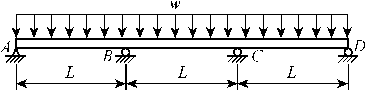
\includegraphics[width=0.7\linewidth]{gfx/three_span_beam}
	\caption{Schematic of three-span continuous beam. Taken from Li, Lü and Yue (2006) \cite{Li2006}}	
	\label{fig:threespanbeam}
\end{figure} 

Consider the three-span beam in figure \ref{fig:threespanbeam}. The associated limit state function is expressed in equation \ref{eq:3_span_beam_g} where the minuend represents the allowable deflection and the subtrahend the maximum deflection. In table \ref{tab:3_span} are the random variables used, which are normally distributed and uncorrelated. The length \(L\) is equal to \(5\) meters.

\begin{equation} \label{eq:3_span_beam_g}
	g(q, E, I) = \frac{L}{360} - 0.0069 \frac{qL^4}{EI}
\end{equation}

\begin{table}
	\myfloatalign
	\begin{tabular}{llrrl}
		\toprule
		\tableheadline{Variable} & \tableheadline{Pdf} & \tableheadline{Mean} & \tableheadline{Std} & \tableheadline{units}\\ \midrule
		\(q\) & Normal & \(10\) & \(0.4\) & \(\frac{kN}{m}\) \\
		\(E\) & Normal & \(2 \times 10^7\) & \(0.5 \times 10^7\) & \(\frac{kN}{m^2}\)\\
		\(I\) & Normal & \(8 \times 10^{-4}\) & \(1.5 \times 10^{-4}\)& \(m^4\) \\
		\bottomrule
	\end{tabular}
	\caption{Random variables considered in section \ref{sec:3_span}}  \label{tab:3_span}
\end{table}

The \ac{MCS} delivers a probability of failure \(P_f = 8.6 \times 10^{-4}\) using \(10^6\) points. On the other hand, \(10^4\) points were used to train the \ac{SVM} model, leaving \(836\) support vectors: \(418\) for each category. A value for \(\gamma\) of \(30\) was chosen resulting in a probability of failure \(P_f = 8.1 \times 10^{-4}\).


\section{A non-linear deflection problem} \label{sec:nonlinear}

Figure \ref{fig:bar} represents a bar whose deflection is expressed by equation \ref{eq:Delta}. Table \ref{tab:nonlinear_deflection} shows the random variables together with their \ac{PDF} including \ac{GEV}, Weibull and Lognormal distributions.

\begin{table}
	\myfloatalign
	\begin{tabular}{llrrl} \toprule
		\tableheadline{Variable} & \tableheadline{PDF}
		& \tableheadline{Mean} & \tableheadline{Std} & \tableheadline{units} \\ \midrule
		\(H\) & GEV & \(5000\) & \(500\) & \(N\)\\
		\(P\) & GEV & \(7000\) & \(500\) & \(N\)\\
		\(I\) & Weibull & \(9 \times 10^{-6}\) & \(100\) & \(-\) \\
		\(L\) & Lognormal & \(4\) & \(0.2\) & \(m\)\\
		\(E\) & Lognormal & \(200\) & \(10\) & \(GPa\)\\
		\(\varphi\) & Lognormal & \(80\) & \(8\) & \(GN \frac{m}{rad}\)\\
		\bottomrule
	\end{tabular}
	\caption{Random variables considered in section \ref{sec:nonlinear}}  \label{tab:nonlinear_deflection}
\end{table}

\begin{figure}
	\myfloatalign
	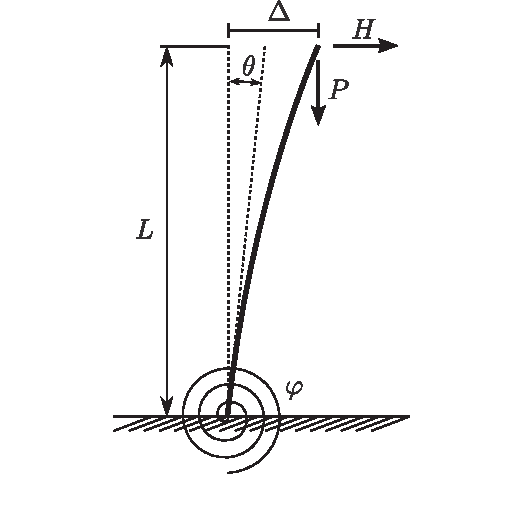
\includegraphics[width=0.75\linewidth]{gfx/bar}
	\caption{Bar studied in section \ref{sec:nonlinear}. Taken from \cite{Hurtado2013} }
	\label{fig:bar}
\end{figure}

The normal and lognormal probability distributions are strongly related since a random variable \(X\) is said to be lognormally distributed if \(y=\ln(x)\) has a normal distribution.

It is therefore usual for a lognormal distribution to be defined in terms of its associated normal distribution. In particular, to produce lognormally distributed random variables in the numpy library, the mean and standard deviation of the associated normal distribution shall be passed, for this purpose equations \ref{eq:LN_to_N} are used.

\begin{align} \label{eq:LN_to_N}
	\mu_N &= \ln \left( \frac{\mu^2_{LN}}{\sqrt{\mu^2_{LN} + \sigma^2_{LN}}} \right)    &    \sigma_N &= \sqrt{\ln \left( 1 + \frac{\sigma^2_{LN}}{\mu^2_{LN}}   \right)}
\end{align}


\begin{equation} \label{eq:Delta}
	\resizebox{.9\hsize}{!}{$
	\Delta = \frac{H}{EI\left ( \frac{P}{EI} \right )^\frac{3}{2}} \left [ \tan \left ( \sqrt{\frac{P}{EI}}L \right ) - \sqrt{\frac{P}{EI}}L + \frac{\varphi^2 \left ( 1 - \sqrt{1 - 4HEI \frac{\tan^2{\left ( \sqrt{ \frac{P}{EI}}L \right )}}{\varphi^2}} \right )^2}{4HEI \tan{\left ( \sqrt{\frac{P}{EI}}L \right )}} \right ]$}
\end{equation}

The bar is said to fail when the tip displacement is greater than 10 cm. The probability of failure obtained through a Monte Carlo simulation with \(10^6\) points is \(P_f = 1.695 \times 10^{-3}\).

Equations \ref{eq:GEV} and \ref{eq:Weibull} describe the \ac{GEV} and Weibull \ac{PDF}s, respectively.

\begin{equation} \label{eq:GEV}
	f(x;\mu, \sigma) = \frac{1}{\sigma} \exp{\left ( \frac{x - \mu}{\sigma} - \exp{\left ( \frac{x - \mu}{\sigma} \right )} \right )}
\end{equation}

\begin{equation} \label{eq:Weibull}
	f(x;\mu, \sigma) = \frac{b}{a^b} x^{b-1} \exp{\left ( - \left ( \frac{x}{a} \right )^b \right )} I_{(0, \infty  )}(x)
\end{equation}

Equation \ref{eq:ITS} is the result of calculating the cumulative distribution function associated with \ac{PDF} and writing it as \(x = f(y)\) (see section \ref{sec:ITS} for more detailed information).

\begin{equation} \label{eq:ITS}
	x = \sigma \ln{\left ( \frac{\mu}{\sigma} \right )} \ln{\left ( -\frac{1}{y-1} \right )}
\end{equation}

Now, in the implementation of the algorithm described in section \ref{sec:algorithm}, \(10^4\) training points were used. The two vectors chosen to initialize the algorithm were taken from the extremes of the population used for the \ac{MCS}. Then, using \(10^6\) vectors to evaluate in the resulting decision function, a failure probability \(P_f=1.607 \times 10^{-3}\) was obtained with \(\gamma=0.9\). In total there were 675 support vectors: 339 safe and 336 unsafe.

\section{Dynamic response of a non-linear oscillator} \label{sec:oscillator}

Consider the nonlinear oscillator shown in figure \ref{fig:oscillator}, which has as limit state function \ref{eq:oscillator_g}. The random variables are generated according to table \ref{tab:oscillator_variables}.

\begin{equation} \label{eq:oscillator_g}
	g (c_1, c_2, m, r, t_1, F_1)= 3r - \left | \frac{2F_1}{m \omega_0^2} \sin{\left ( \frac{\omega_0 t_1}{2} \right )} \right |
\end{equation}

\begin{equation} \label{eq:omega_0}
	\omega_0 = \sqrt{\frac{c_1 + c_2}{m}}
\end{equation}

The Monte Carlo simulation was performed with \(10^6\) points and gave a probability of failure  \(P_f = 2.83 \times 10^{-2}\). The \ac{SVM} model was trained with \(10^4\) uniformly distributed points and the points \((x_1, x_2)\) chosen to start the algorithm were taken from the extremes of the \ac{MCS}. A total of \(1414\) support vectors were used: \(709\) safe and \(705\) unsafe.

In this case a \( \gamma=1/6\) was used. Finally, \(10^6\) points were evaluated in the decision function and a probability of \(2.85 \times 10^{-2}\) was obtained.

\begin{figure}
	\myfloatalign
	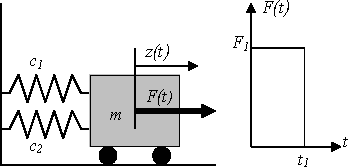
\includegraphics[width=0.7\linewidth]{gfx/oscillator}
	\caption[Non-linear oscillator]{ Non-linear oscillator – system definition and applied load. Taken from \cite{Schueremans2005}}
	\label{fig:oscillator}
\end{figure}

\begin{table}
	\myfloatalign
	\begin{tabular}{llrrl} \toprule
		\tableheadline{Variable} & \tableheadline{PDF}
		& \tableheadline{Mean} & \tableheadline{Std} \\ \midrule
		\(m\)   & Normal & \(1.0\) & \(0.05\) \\
		\(c_1\) & Normal & \(1.0\) & \(0.10\) \\
		\(c_2\) & Normal & \(0.1\) & \(0.01\) \\
		\(r\)   & Normal & \(0.5\) & \(0.05\) \\
		\(F_1\) & Normal & \(1.0\) & \(0.20\) \\
		\(t_1\) & Normal & \(1.0\) & \(0.20\) \\
		\bottomrule
	\end{tabular}
	\caption{Random variables considered in section \ref{sec:oscillator}}  \label{tab:oscillator_variables}
\end{table}

\section{Final Thoughts}

Support vector machines are simple, elegant and deliver remarkable results using less computational overhead than the Monte Carlo method. The algorithm tested here makes efficient use of samples and avoids unnecessary calls to the limit state function which sometimes requires intensive computation.
